\documentclass{article}
\RequirePackage{etex}
\usepackage{geometry}
\geometry{a4paper, margin = 1.0in}
\usepackage[utf8]{inputenc}
\usepackage[english]{babel}
\usepackage[dvipsnames]{xcolor}
\usepackage{framed,graphicx}
\usepackage{hyperref}
\hypersetup{colorlinks=true,linkcolor=blue,filecolor=magenta,urlcolor=Cerulean,citecolor=SkyBlue}
\usepackage{listings}
\usepackage{mathtools}
\usepackage{amsfonts,amsthm,mathrsfs}
\usepackage{paracol}
\usepackage{wrapfig}
\usepackage[nottoc]{tocbibind}
\usepackage{natbib}
\usepackage[font={scriptsize,it}]{caption}
\usepackage{float}
\usepackage{multicol}
\usepackage[font={scriptsize}]{subcaption}
\usepackage{pgfplots,tikz,tkz-euclide}
\usetikzlibrary{calc,patterns,angles,quotes,arrows,arrows.meta,shapes,shapes.geometric,cd,hobby,positioning}
\usetkzobj{all}
\pgfplotsset{compat=1.9}
\usepackage[toc,acronym,nogroupskip]{glossaries}
\usepackage{enumitem}
\usepackage{upgreek}
\graphicspath{{images/}}
%-------------Tikz Presets----------%
\pgfdeclareradialshading{myring}{\pgfpointorigin}{
color(0cm)=(transparent!0);
color(5mm)=(pgftransparent!50);
color(1cm)=(pgftransparent!100)}
\pgfdeclarefading{ringo}{\pgfuseshading{myring}}
%------------Theorem Styles---------%
\newtheoremstyle{mystyle}{\topsep}{\topsep}{}{}{\bfseries}{}{.5em}{}
\theoremstyle{mystyle}
\newtheorem{theorem}{Theorem}[section]
\newtheorem{definition}{Definition}[section]
\newtheorem{lemma}{Lemma}[section]
\newtheorem{corollary}{Corollary}[section]
\newtheorem{proposition}{Proposition}[section]
\newtheorem{example}{Example}[section]
\newtheorem{problem}{Problem}[section]
\newtheorem{question}{Question}[section]
\newtheorem{remark}{Remark}[section]
\newtheorem{properties}{Properties}[section]
\newtheorem{notation}{Notation}[section]
\newtheorem{axiom}{Axiom}[section]
\newtheorem*{theorem*}{Theorem}
\newtheorem*{definition*}{Definition}
\newtheorem*{properties*}{Properties}
\newtheorem*{remark*}{Remark}
%--------Declared Math Operators----%
\DeclareMathOperator{\Refl}{Refl}
\DeclareMathOperator{\Span}{Span}
\DeclareMathOperator{\sgn}{sgn}
\DeclareMathOperator{\multideg}{mutlideg}
\DeclareMathOperator{\LC}{LC}
\DeclareMathOperator{\LT}{LT}
\DeclareMathOperator{\LM}{LM}
\DeclareMathOperator{\LCM}{LCM}
\DeclareMathOperator{\Mon}{Mon}
\DeclareMathOperator{\Spec}{Spec}
\DeclareMathOperator{\proj}{proj}
\DeclareMathOperator{\comp}{comp}
\DeclareMathOperator{\sinc}{sinc}
%-------------New Commands----------%
\DeclarePairedDelimiter\norm{\lVert}{\rVert}
\DeclarePairedDelimiter\ceil{\lceil}{\rceil}
\DeclarePairedDelimiter\floor{\lfloor}{\rfloor}
\definecolor{shadecolor}{gray}{0.9}
\renewcommand*{\glstextformat}[1]{\textcolor{RoyalBlue}{#1}}
\renewcommand{\glsnamefont}[1]{\textbf{#1}}
\renewcommand\labelitemii{$\circ$}
\renewcommand\thesubfigure{\arabic{section}.\arabic{figure}.\arabic{subfigure}}
%---------------GLOSSARY------------%
\makeglossaries
\loadglsentries{glossary}
\loadglsentries{acronym}

\title{Notes on Mathematics}
\author{Ryan Maguire}
\date{\vspace{-5ex}}
\begin{document}
\maketitle
\tableofcontents
\setlength{\parindent}{0em}
\setlength{\parskip}{0em}
\section{Atmospheric Occultation}
\subsection{Titan Geometry}
\begin{figure}[H]
	\centering
	\begin{subfigure}[b]{0.49\textwidth}
	    \centering
        \resizebox{\textwidth}{!}{
        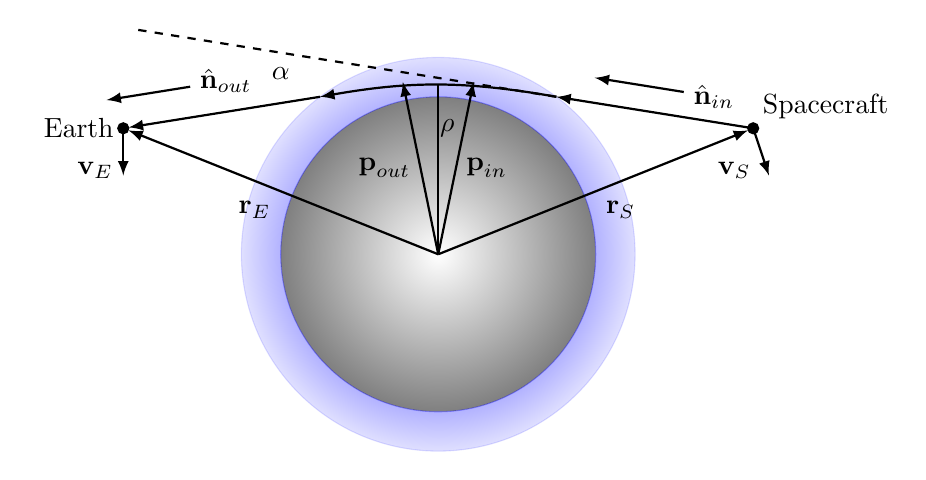
\begin{tikzpicture}[axis/.style={very thick, ->, >=stealth'},
            important line/.style={thick},
            dashed line/.style={dashed, thin},
            pile/.style={thick,->, >=stealth', shorten <=2pt,shorten>=2pt},every node/.style={color=black}]
            \coordinate (S)  at (4,1.6);
            \coordinate (E)  at (-4,1.6);
            \coordinate (O)  at (0,0);
            \coordinate (p1) at (-1.5,2);
            \coordinate (p2) at (1.5,2);
            \coordinate (P) at (0,2.2);
            \shade [even odd rule,inner color=white,outer color=gray] (0, 0) circle (2cm);
            \filldraw[even odd rule,blue ,path fading=ringo] (0,0) circle (25mm) (0,0) circle (2cm);
            \filldraw[black] (E) circle (2pt) node[left] {Earth};
            \filldraw[black] (S) circle (2pt) node[above right] {Spacecraft};
        \begin{scope}[>={latex[black]},every edge/.style={draw=black,thick}]
            \path [->] (S) edge (p2);
            \path [->] (p2) edge[bend right=10] (p1);
            \path [->,shorten >=2pt,shorten <=0cm,->] (p1) edge (E);
            \path [->] (O) edge node[right] {$\textbf{p}_{in}$} (0.45,2.18874);
            \path [->] (O) edge node[left] {$\textbf{p}_{out}$} (-0.45,2.18874);
            \path [->,shorten >=2pt,shorten <=0cm,->] (O) edge node[below left] {$\mathbf{r}_{E}$} (E);
            \path [->,shorten >=2pt,shorten <=0cm,->] (O) edge node[below right] {$\mathbf{r}_{S}$} (S);
            \path [->] (S) edge node[below left] {$\mathbf{v}_{S}$} (4.2,1);
            \path [->] (E) edge node[below left] {$\mathbf{v}_{E}$} (-4,1);
            \path (O) edge (0,2.15);
        \end{scope}
            \node (nin) at (3.5,2) {$\hat{\mathbf{n}}_{in}$};
            \node (nout) at (-2.7,2.2) {$\hat{\mathbf{n}}_{out}$};
            \draw[>={latex[black]},thick,shorten >=1cm,shorten <=0cm,->] (nin) -- +($(p2)-(S)$);
            \draw[>={latex[black]},thick,shorten >=1cm,shorten <=0cm,->] (nout) -- +($(E)-(p1)$);
            \draw[thick,dashed] (p2) -- ($(S)!8cm!(p2)$);
            \node at (-2,2.3) {$\alpha$};
            \node at (-0.1,1.6) [right] {$\rho$};
        \end{tikzpicture}}
    	\caption{Geometry of an Occultation of Titan}
	    \label{fig:math_titan_geom_vec}
    \end{subfigure}
    \begin{subfigure}[b]{0.49\textwidth}
        \centering
        \resizebox{\textwidth}{!}{
        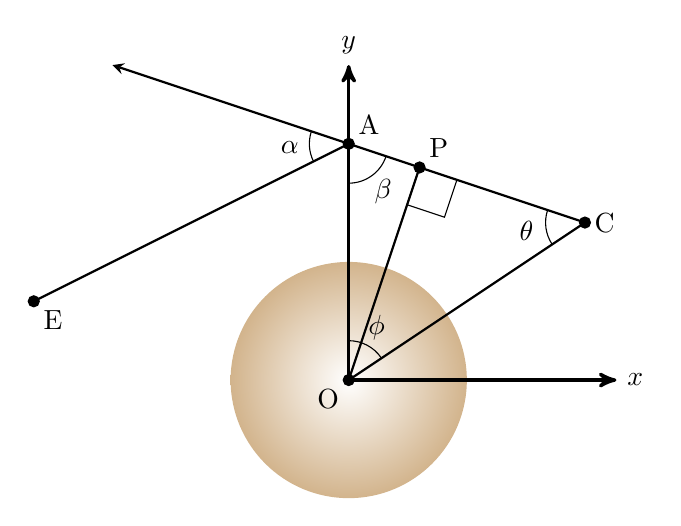
\begin{tikzpicture}[axis/.style={very thick, ->, >=stealth'},important line/.style={thick},
        dashed line/.style={dashed, thin},pile/.style={thick,->, >=stealth', shorten <=2pt,shorten>=2pt},every node/.style={color=black}]
        \coordinate (O) at (0,0) {};
        \coordinate (E) at (-4,1) {};
        \coordinate (C) at (3,2) {};
        \coordinate (A) at (0,3) {};
        \coordinate (P) at (0.9,2.7) {};
        \coordinate (Space) at (-3,4) {};
        \shade[inner color=white,outer color=Tan] (0,0) circle (1.5);
        \draw[axis] (0,0) -> (0,4)node(yline)[above] {$y$};
        \draw[axis] (0,0) -> (3.4,0)node(xline)[right] {$x$};
        \draw[thick] (0,0) -- (3,2);
        \filldraw[black] (3,2) circle (2pt) node[right] {C};
        \filldraw[black] (0,0) circle (2pt) node[below left] {O};
        \draw[thick, ->,>=stealth] (3,2) -- (-3,4);
        \filldraw[black] (0,3) circle (2pt) node[above right] {A};
        \draw[thick] (0,3) -- (-4,1);
        \filldraw[black] (-4,1) circle (2pt) node[below right] {E};
        \pic [draw=black, -, "$\alpha$", angle eccentricity=1.5] {angle = Space--A--E};
        \pic [draw=black, -, "$\beta$", angle eccentricity=1.5] {angle = O--A--C};
        \pic [draw=black, -, "$\theta$", angle eccentricity=1.5] {angle = A--C--O};
        \pic [draw=black, -, "$\phi$", angle eccentricity=1.5] {angle = C--O--A};
        \draw[thick] (0,0) -- (0.9,2.7);
        \filldraw[black] (0.9,2.7) circle (2pt) node[above right] {P};
        \tkzMarkRightAngle[draw=black,size=0.5](O,P,C);
    \end{tikzpicture}}
    \caption{Geometry of the Bending Angle}
    \label{fig:math_geo_bending_angle}
    \end{subfigure}
\end{figure}
The following definitions are used:
\begin{enumerate}[itemsep=0pt]
    \begin{multicols}{2}
        \item $O$ is Titan.
        \item $E$ is Earth.
        \item $C$ is Cassini.
        \item $\mathbf{r}_{E} = \overrightarrow{OE}$
        \item $\mathbf{v}_{E} = \frac{d}{dt}\mathbf{r}_{E}$
        \item $\mathbf{r}_{S} = \overrightarrow{OC}$
        \item $\mathbf{v}_{S} = \frac{d}{dt}\mathbf{r}_{S}$
        \item $\mathbf{p}_{in}$ is the projection of $O$ onto $\overline{AC}$
        \item $\mathbf{p}_{out}$ is the projection of $O$ onto $\overline{EA}$
        \item $\alpha$ is the bending angle ($\pi-\angle EAC$)
        \item $\hat{\mathbf{n}}_{in}$ is the direction of the emission.
        \item $\hat{\mathbf{n}}_{out}$ is the direction of the reception.
        \item The ray plane is the plane $OEC$
        \item $\phi = \angle OAC$
        \item $\theta = \angle ACO$
        \item $\beta = \angle AOC$
    \end{multicols}
    \vspace{-3ex}
    \item $A$ is the intersection of the lines starting at $C$ and $E$, parallel to $\hat{\mathbf{n}}_{in}$ and $\hat{\mathbf{n}}_{out}$, respectively.
\end{enumerate}
The following assumptions are made:
\begin{enumerate}
    \begin{multicols}{2}
        \item $\angle OAE = \angle OAC$
        \item $A$ lies in the plane $OEC$
    \end{multicols}
\end{enumerate}
\begin{theorem}
\label{theorem:ray_plane_perp_to_r_e_cross_r_s}
The ray plane is perpendicular to $\hat{\mathbf{z}} = \frac{\mathbf{r}_{S}\times \mathbf{r}_{E}}{\norm{\mathbf{r}_{S}\times \mathbf{r}_{E}}}$
\end{theorem}
\begin{proof}
As the ray plane is the plane $OEC$, $\mathbf{r}_{S}$ and $\mathbf{r}_{E}$ lie parallel to this plane. Moreover, during an occultation, $\mathbf{r}_{S}$ and $\mathbf{r}_{E}$ are not parallel and therefore $OEC$ is uniquely determined by $\mathbf{r}_{E}$, $\mathbf{r}_{S}$, and the point $O$. But $\hat{\mathbf{z}} = \frac{\mathbf{r}_{S}\times \mathbf{r}_{E}}{\norm{\mathbf{r}_{S}\times \mathbf{r}_{E}}}$ is perpendicular to both $\mathbf{r}_{E}$ and $\mathbf{r}_{S}$. Therefore $\hat{\mathbf{z}}$ is perpendicular to the ray plane.
\end{proof}
\begin{theorem}
\label{theorem:r_e_dot_p_out_equal_p_out_square}
$\mathbf{r}_{E}\cdot \mathbf{p}_{out} = \norm{\mathbf{p}_{out}}^2$
\end{theorem}
\begin{proof}
$\mathbf{p}_{out}$ is the projection of the $O$ onto $\overline{EA}$. But $\overline{EA}$ lies parallel to $\hat{\mathbf{n}}_{out}$, and therefore $\mathbf{p}_{out}$ and $\hat{\mathbf{n}}_{out}$ are orthogonal, and thus $\mathbf{p}_{out}\cdot\hat{\mathbf{n}}_{out}=0$. Moreoever, $\mathbf{r}_{E} = \mathbf{p}_{out}+(\mathbf{r}_{E}\cdot \hat{\mathbf{n}}_{out}) \hat{\mathbf{n}}_{out}$. But then:
\begin{align*}
    \mathbf{p}_{out}\cdot \mathbf{r}_{E} &= \mathbf{p}_{out}\cdot\big(\mathbf{p}_{out}+(\mathbf{r}_{E}\cdot \hat{\mathbf{n}}_{out})\hat{\mathbf{n}}_{out}\big)\\
    \Rightarrow \mathbf{p}_{out}\cdot \mathbf{r}_{E} &= \mathbf{p}_{out}\cdot \mathbf{p}_{out} + (\mathbf{r}_{E}\cdot \hat{\mathbf{n}}_{out}) \mathbf{p}_{out}\cdot \hat{\mathbf{n}}_{out}\\
    \Rightarrow \mathbf{p}_{out}\cdot \mathbf{r}_{E} &= \mathbf{p}_{out}\cdot \mathbf{p}_{out}
\end{align*}
Therefore $\mathbf{p}_{out}\cdot \mathbf{r}_{E} = \norm{\mathbf{p}_{out}}^2$
\end{proof}
\begin{theorem}
$\alpha = \cos^{-1}(\hat{\mathbf{n}}_{in}\cdot \hat{\mathbf{n}}_{out})$
\end{theorem}
\begin{proof}
By definition, $\alpha = \pi - \angle EAC$. But $\hat{\mathbf{n}}_{out}$ lies parallel to $\overrightarrow{AE}$, and $-\hat{\mathbf{n}}_{in}$ lies parallel to $\overrightarrow{AC}$. Therefore:
\begin{equation*}
-\hat{\mathbf{n}}_{out}\cdot \hat{\mathbf{n}}_{in} = \hat{\mathbf{n}}_{out}\cdot (-\hat{\mathbf{n}}_{in}) = \norm{\hat{\mathbf{n}}_{out}}\norm{-\hat{\mathbf{n}}_{in}}\cos(\angle EAC)
\end{equation*}
But $\hat{\mathbf{n}}_{in}$ and $\hat{\mathbf{n}}_{out}$ are unit vectors, and therefore $\norm{\hat{\mathbf{n}}_{out}} = \norm{-\hat{\mathbf{n}}_{in}} = 1$. Therefore:
\begin{equation*}
    \angle EAC = \cos^{-1}(-\hat{\mathbf{n}}_{out}\cdot\hat{\mathbf{n}}_{in})
\end{equation*}
But $\alpha = \pi - \angle EAC$, and $\cos^{-1}(-x) = \pi - \cos^{-1}(x)$. Therefore:
\begin{equation*}
    \alpha = \pi - \angle EAC = \pi - \big(\pi - \cos^{-1}(\hat{\mathbf{n}}_{out}\cdot \hat{\mathbf{n}}_{in})\big) = \cos^{-1}(\hat{\mathbf{n}}_{out}\cdot \hat{\mathbf{n}}_{in})
\end{equation*}
\end{proof}
\begin{theorem}
$\theta = \cos^{-1}\big(\frac{(-\mathbf{r}_{S})\cdot \hat{\mathbf{n}}_{in}}{\norm{\mathbf{r}_{S}}}\big)$
\end{theorem}
\begin{proof}
For $\theta = \angle OCA$. But $\hat{\mathbf{n}}_{in}$ is parallel with $\overrightarrow{CA}$, and $(-\mathbf{r}_{S})$ is parallel with $\overrightarrow{CO}$. Therefore:
\begin{align*}
    (-\mathbf{r}_{S})\cdot \hat{\mathbf{n}}_{in} &= \norm{(-\mathbf{r}_{S})}\norm{\hat{\mathbf{n}}_{in}}\cos(\theta)\\
    \Rightarrow \theta &= \cos^{-1}\bigg(\frac{(-\mathbf{r}_{S})\cdot \hat{\mathbf{n}}_{in}}{\norm{\mathbf{r}_{S}}}\bigg)
\end{align*}
\end{proof}
\begin{theorem}
$\beta = \pi - \frac{1}{2}\cos^{-1}\bigg(\frac{\mathbf{r}_{s}\cdot \mathbf{r}_{E}}{\norm{\mathbf{r}_{s}}\norm{\mathbf{r}_{E}}}\bigg) - \frac{1}{2}\cos^{-1}\bigg(\frac{\mathbf{r}_{E}\cdot \hat{\mathbf{n}}_{out}}{\norm{\mathbf{r}_{E}}}\bigg) - \frac{1}{2}\cos^{-1}\bigg(\frac{(-\mathbf{r}_{s})\cdot \hat{\mathbf{n}}_{in}}{\norm{\mathbf{r}_{s}}}\bigg)$
\end{theorem}
\begin{proof}
The sum of the angles in $OEAC$ is $2\pi$. But $\angle OAE = \angle OAC = \phi$, and therefore:
\begin{align*}
    2\beta &=\angle EAC \\
    \Rightarrow 2\pi &= 2\beta + \angle AEO + \angle EOC + \angle OCA\\
    \Rightarrow \beta &= \pi - \frac{\angle AEO}{2}-\frac{\angle EOC}{2}-\frac{\angle OCA}{2}
\end{align*}
But:
\begin{align*}
(-\hat{\mathbf{n}}_{out})\cdot (-\hat{\mathbf{r}}_{E}) &= \norm{\mathbf{r}_{E}}\cos(\angle AEO)\\
\Rightarrow \angle AEO &= \cos^{-1}\bigg(\frac{\hat{\mathbf{n}}_{out}\cdot \mathbf{r}_{E}}{\norm{\mathbf{r}_{E}}}\bigg)
\end{align*}
Also:
\begin{align*}
    \mathbf{r}_{E}\cdot \mathbf{r}_{S} &= \norm{\mathbf{r}_{E}}\norm{\mathbf{r}_{S}}\cos(\angle EOC)\\
    \Rightarrow \angle EOC &= \cos^{-1}\bigg(\frac{\mathbf{r}_{E}\cdot \mathbf{r}_{S}}{\norm{\mathbf{r}_{E}}\norm{\mathbf{r}_{S}}}\bigg)
\end{align*}
But $\angle OCA = \theta = \cos^{-1}\big(\frac{(-\mathbf{r}_{S})\cdot \hat{\mathbf{n}}_{in}}{\norm{\mathbf{r}_{S}}}\big)$. Therefore:
\begin{equation*}
\beta = \pi - \frac{1}{2}\cos^{-1}\bigg(\frac{\mathbf{r}_{s}\cdot \mathbf{r}_{E}}{\norm{\mathbf{r}_{s}}\norm{\mathbf{r}_{E}}}\bigg) - \frac{1}{2}\cos^{-1}\bigg(\frac{\mathbf{r}_{E}\cdot \hat{\mathbf{n}}_{out}}{\norm{\mathbf{r}_{E}}}\bigg) - \frac{1}{2}\cos^{-1}\bigg(\frac{(-\mathbf{r}_{s})\cdot \hat{\mathbf{n}}_{in}}{\norm{\mathbf{r}_{s}}}\bigg)
\end{equation*}
\end{proof}
\begin{theorem}
$\alpha = \pi - 2\beta$
\end{theorem}
\begin{proof}
$\alpha$ and $\angle EAC$ are supplementary to the ray $\overrightarrow{CA}$, and therefore $\alpha + \angle EAC = \pi$. But $\angle EAC = \angle EAC + \angle OAC = 2\beta$. Therefore $\alpha + 2\beta = \pi$. Thus, $\alpha = \pi - 2\beta$.
\end{proof}
\begin{theorem}
$\theta = \frac{\pi}{2}+ \frac{\alpha}{2}-\phi$
\end{theorem}
\begin{proof}
As the angles of a triangle sum to $\pi$, $\theta+\beta+\phi = \pi$. But $\alpha = \pi - 2\beta \Rightarrow \beta = \frac{\pi}{2}-\frac{\alpha}{2}$. So we have:
\begin{align*}
    \theta+\phi+\beta &=\pi \\
    \Rightarrow \theta+\phi+\frac{\pi}{2}-\frac{\alpha}{2} &= \pi\\
    \Rightarrow \theta &= \frac{\pi}{2} +\frac{\alpha}{2}-\phi
\end{align*}
\end{proof}
\begin{theorem}
$\phi = \frac{1}{2}\cos^{-1}\bigg(\frac{\mathbf{r}_{s}\cdot \mathbf{r}_{E}}{\norm{\mathbf{r}_{s}}\norm{\mathbf{r}_{E}}}\bigg) + \frac{1}{2}\cos^{-1}\bigg(\frac{\mathbf{r}_{E}\cdot \hat{\mathbf{n}}_{out}}{\norm{\mathbf{r}_{E}}}\bigg) - \frac{1}{2}\cos^{-1}\bigg(\frac{(-\mathbf{r}_{s})\cdot \hat{\mathbf{n}}_{in}}{\norm{\mathbf{r}_{s}}}\bigg) $
\end{theorem}
\begin{proof}
For:
\begin{align*}
    \pi &=\beta+\theta+\phi\\
    \theta &= \cos^{-1}\big(\frac{(-\mathbf{r}_{S})\cdot\hat{\mathbf{n}}_{in}}{\norm{\mathbf{r}_{S}}}\big)\\
    \beta &= \pi-\frac{1}{2}\cos^{-1}\bigg(\frac{\mathbf{r}_{s}\cdot \mathbf{r}_{E}}{\norm{\mathbf{r}_{s}}\norm{\mathbf{r}_{E}}}\bigg) - \frac{1}{2}\cos^{-1}\bigg(\frac{\mathbf{r}_{E}\cdot \hat{\mathbf{n}}_{out}}{\norm{\mathbf{r}_{E}}}\bigg) - \frac{1}{2}\cos^{-1}\bigg(\frac{(-\mathbf{r}_{s})\cdot \hat{\mathbf{n}}_{in}}{\norm{\mathbf{r}_{s}}}\bigg)\\
    \Rightarrow \phi & = \frac{1}{2}\cos^{-1}\bigg(\frac{\mathbf{r}_{s}\cdot \mathbf{r}_{E}}{\norm{\mathbf{r}_{s}}\norm{\mathbf{r}_{E}}}\bigg) + \frac{1}{2}\cos^{-1}\bigg(\frac{\mathbf{r}_{E}\cdot \hat{\mathbf{n}}_{out}}{\norm{\mathbf{r}_{E}}}\bigg) - \frac{1}{2}\cos^{-1}\bigg(\frac{(-\mathbf{r}_{s})\cdot \hat{\mathbf{n}}_{in}}{\norm{\mathbf{r}_{s}}}\bigg)
\end{align*}
\end{proof}
\begin{theorem}
\label{theorem:impact_parameter_p_closed_form_solution}
$p = \norm{\mathbf{p}_{in}} = \norm{\mathbf{r}_{S}}\cos(\phi - \frac{\alpha}{2})$
\end{theorem}
\begin{proof}
As $P$ is the orthogonal projection of $O$ onto $\overline{CA}$, $\angle OPC = \frac{\pi}{2}$. But then:
\begin{equation*}
    |\overline{OP}| = |\overline{OC}|\sin(\angle OCP)
\end{equation*}
But $|\overline{OP}| = \norm{\mathbf{p}_{in}}$, $|\overline{OC}| = \norm{\mathbf{r}_{S}}$, and $\angle OCP = \theta$. Therefore:
\begin{equation*}
    \norm{\mathbf{p}_{in}} = \norm{\mathbf{r}_{S}}\sin(\theta)
\end{equation*}
But $\theta = \frac{\pi}{2} + \frac{\alpha}{2} - \phi$, and $\sin(\frac{\pi}{2}+x) = \cos(x)$. Therefore:
\begin{equation*}
    \norm{\mathbf{p}_{in}} = \norm{\mathbf{r}_{S}}\cos\big(\frac{\alpha}{2} - \phi\big)
\end{equation*}
\end{proof}
\begin{theorem}
$\norm{\mathbf{p}_{in}} = |\overline{OA}|\sin(\beta)$
\end{theorem}
\begin{proof}
For $\overline{OP}$ is perpendicular to $\overline{CA}$, and therefore $\Delta OPA$ is a right-angled triangle, and $\overline{OA}$ is the hypotenuse. Moreoever $\angle PAO = \beta$. But then:
\begin{align*}
|\overline{OP}| &= |\overline{OA}|\sin(\angle PAO)\\
\Rightarrow |OP| &= |\overline{OA}|\sin(\beta)
\end{align*}
But $\norm{\mathbf{p}_{in}} = |\overline{OP}|$, and thus $\norm{\mathbf{p}_{in}} = |OA|\sin(\beta)$
\end{proof}
\begin{theorem}
\label{theorem:p_out_equals_p_in}
$\norm{\mathbf{p}_{in}} = \norm{\mathbf{p}_{out}}$
\end{theorem}
\begin{proof}
For $\angle OAE = \angle OAC = \beta$, and thus:
\begin{equation*}
    \norm{\mathbf{p}}_{out} = |\overline{OA}|\sin(\angle OAE) = |\overline{OA}|\sin(\beta)=\norm{\mathbf{p}}_{in}
\end{equation*}
\end{proof}
\section{Ring Occultation}
\subsection{Some Useful Results}
\begin{definition}
The ${p}$ norm of an integrable function $f$ is $\norm{f}_{p} = \big(\int_{-\infty}^{\infty}|f|^{p}dx\big)^{1/p}$
\end{definition}
\begin{definition}
$L^{p}$ is the set $\{f:\mathbb{R}\rightarrow \mathbb{R}:\norm{f}_{p}<\infty\}$
\end{definition}
\begin{definition}
The supremum norm of an integrable function is $\norm{f}_{\infty} = \underset{p\rightarrow \infty}{\lim}\norm{f}_{p}$
\end{definition}
\begin{definition}
$L^{\infty}$ is the set of bounded integrable functions.
\end{definition}
\begin{theorem}
If $f$ is integrable and bounded, then $\norm{f}_{\infty} = \sup(\{f(x):x\in\mathbb{R}\})$
\end{theorem}
Where $\sup$ means supremum, and in most situations this simply means the maximum value. If $f(x) = e^{-x^2}$, then $\sup(\{f(x):x\in\mathbb{R}\}) = 1$, for this is the largest value attained by $f$. For most of the mathematics involved we deal exclusively with $L^{1},L^{2},$ and $L^{\infty}$ functions. We will use these types of functions in our developement of the theory of convolutions. First, a brief discussion on complex analysis.
\begin{definition}
The complex numbers are the set $\mathbb{C} = \{(x,y):x,y\in\mathbb{R}\}$ with the following arithmetic:
\begin{enumerate}
    \item $(a,b) + (c,d) = (a+c,b+d)$
    \item $(a,b)\cdot (c,d) = (ac - bd,ad+bc)$
    \item $r(a,b) = (ra,rb)$
\end{enumerate}
\end{definition}
It is often both useful and intuitive to think of a complex number $z=(a,b)$ as $z=a+ib$ where $i$ is the imaginary unit defined by $i^2 = -1$. Several problems arise from this, such as ambiguity. For if $i^2 = -1$, then $(-i)^2 = -1$, so the imaginary unit is not unique. Thinking of the complex numbers as ordered pairs (Elements of the Euclidean plane) with the aforementioned arithmetic rids of this problem, and it also allows one to define the principle $n^{th}$ root of a complex number.
\begin{definition}
The modulus of a complex number $z = (a,b)$, denoted $|z|$, is the real number $\sqrt{a^2+b^2}$.
\end{definition}
\begin{theorem}
If $z$ is a complex number, then there is a unique $\theta \in [0,2\pi)$ such that $z =|z|(\cos(\theta),\sin(\theta))$
\end{theorem}
\begin{proof}
Let $z=(a,b)$ be a complex number. If $b=0$ and $a\geq 0$ then $z = a(\cos(0),\sin(0))$. If $b=0$ and $a<0$, THEN $z=a(\cos(\pi),\sin(\pi))$. If $b\ne 0$, then:
\begin{equation*}
    z = (a,b) = |z|(\frac{a}{|z|},\frac{b}{|z|})
\end{equation*}
\end{proof}
\begin{theorem}
$\sqrt{i} = \frac{1+i}{2}$
\end{theorem}
\begin{proof}
For $i = e^{i\frac{\pi}{2}}$, and thus $\sqrt{i} = e^{i\frac{\pi}{4}} = \cos(\frac{\pi}{4})+i\sin(\frac{\pi}{4}) = \frac{1+i}{\sqrt{2}}$
\end{proof}
\begin{theorem}
If $a+ib$ is a complex number, and $(a,b) \ne (0,0)$, then $\frac{1}{a+ib} = \frac{a-ib}{a^2+b^2}$.
\end{theorem}
\begin{proof}
If $(a,b)\ne (0,0)$, then $a^2+b^2>0$, so $\frac{a-ib}{a^2+b^2}$ is a complex number. But:
\begin{equation*}
    (a+ib)\cdot \frac{a-ib}{a^2+b^2} = \frac{(a+ib)(a-ib)}{a^2+b^2} = \frac{a^2+b^2}{a^2+b^2} = 1
\end{equation*}
From the uniqueness of inverses, $\frac{1}{a+ib} = \frac{a-ib}{a^2+b^2}$.
\end{proof}
\begin{theorem}
$\int_{-\infty}^{\infty}e^{-x^2}dx = \sqrt{\pi}$.
\end{theorem}
\begin{proof}
Convergence can be shown, for $0 < e^{-x^2} \leq \frac{1}{1+x^2}$ for all $x\in \mathbb{R}$. Therefore:
\begin{equation*}
0<\int_{-\infty}^{\infty} e^{-x^2}dx \leq \int_{-\infty}^{\infty} \frac{1}{1+x^2}dx = \tan^{-1}(x)\big|_{-\infty}^{\infty} = \pi
\end{equation*}
Let $\mathcal{I} = \int_{-\infty}^{\infty} e^{-x^2}dx$. Then:
\begin{equation*}
    \mathcal{I}^2 = \bigg(\int_{-\infty}^{\infty}e^{-x^2}dx\bigg)\bigg(\int_{-\infty}^{\infty}e^{-y^2}dy\bigg) = \int_{-\infty}^{\infty}\int_{-\infty}^{\infty}e^{-(x^2+y^2)}dxdy
\end{equation*}
Switching from Cartesian to Polar coordinates, we have:
\begin{equation*}
    \int_{0}^{2\pi}\int_{0}^{\infty} re^{-r^2}dr = 2\pi \int_{0}^{\infty}re^{-r^2}dr
\end{equation*}
Let $u = r^2$. Then we have $du = 2rdr$, so the integral becomes $\pi \int_{0}^{\infty} e^{-u}du = \pi$. Hence, $\mathcal{I}^2 = \pi$, and therefore $\mathcal{I} = \pm \sqrt{\pi}$. But $\mathcal{I} > 0$, so $\mathcal{I} = \sqrt{\pi}$. Therefore, $\int_{-\infty}^{\infty}e^{-x^2}dx = \sqrt{\pi}$. 
\end{proof}
\begin{theorem}
For all $x\in \mathbb{R}$, $e^{ix} = \cos(x)+i\sin(x)$.
\end{theorem}
\begin{proof}
For $e^{ix}$ is the solution to $y' = iy, y(0) = 1$. But:
\begin{equation*}
    \frac{d}{dx}\big(\cos(x)+i\sin(x)\big) = -\sin(x)+i\cos(x) = i\big(\cos(x)+i\sin(x)\big)
\end{equation*}
Moreover, $\cos(0)+i\sin(0) = 1$. Therefore $\cos(x)+i\sin(x)$ satisfies the same differential equation. From uniqueness of solutions, $e^{ix} = \cos(x)+i\sin(x)$.
\end{proof}
\begin{theorem}
$\int_{-\infty}^{\infty} e^{i\frac{\pi}{2}x^2}dx = 1+i$
\end{theorem}
\begin{proof}
Let $x = i\sqrt{\frac{2}{i\pi}}z$. Then $i\frac{\pi}{2}x^2 = -z^2$, and $dx = i\sqrt{\frac{2}{i\pi}}dz$. So we have:
\begin{equation*}
    \int_{-\infty}^{\infty}e^{i\frac{\pi}{2}x^2}dx = i\sqrt{\frac{2}{i\pi}}\int_{-\infty}^{\infty} e^{-z^2}dz    
\end{equation*}
But $\sqrt{i} = \frac{1+i}{\sqrt{2}}$, and $\frac{1}{\sqrt{i}} = \frac{\sqrt{2}}{1+i} = \frac{1-i}{\sqrt{2}}$, from the previous theorems. Therefore:
\begin{equation*}
    i\sqrt{\frac{2}{\pi}}\frac{1-i}{\sqrt{2}}\int_{-\infty}^{\infty}e^{-z^2}dz = (1+i)\frac{1}{\sqrt{\pi}}\int_{-\infty}^{\infty}e^{-z^2}dz
\end{equation*}
But $\int_{-\infty}^{\infty}e^{-z^2}dz = \sqrt{\pi}$. Thus, we have $1+i$.
\end{proof}
\begin{theorem}
$\mathcal{F}\big(e^{i\frac{\pi}{2}(\frac{\rho}{F})^2}\big) = (1+i)Fe^{-i2\pi F^2 \xi^2}$
\end{theorem}
\begin{proof}
For:
\begin{equation*}
    \mathcal{F}\big(e^{i\frac{\pi}{2} \big(\frac{\rho}{F}\big)^2}\big) = \int_{-\infty}^{\infty} e^{i\frac{\pi}{2}\big(\frac{\rho}{F}\big)^2}e^{-2\pi i \rho \xi}d\rho = \int_{-\infty}^{\infty} e^{i\frac{\pi}{2}\big(\frac{\rho}{F}\big)^2-2\pi i \rho \xi}d\rho = \int_{-\infty}^{\infty} e^{i\frac{\pi}{2F^2}\big[\rho^2-4F^2\rho \xi\big]}d\rho    
\end{equation*}
Completing the square, we get $(\rho - 2F^2 \xi)^2 - 4F^4\xi^2$. So, the integral becomes:
\begin{equation*}
    \int_{-\infty}^{\infty} e^{i\frac{\pi}{2F^2}(\rho - 2F^2\xi)^2}e^{-2\pi i F^2 \xi^2}d\rho = e^{-2\pi i F^2 \xi^2}\int_{-\infty}^{\infty} e^{i\frac{\pi}{2F^2}(\rho - 2F^2\xi)^2}d\rho
\end{equation*}
Let $u = \rho - 2F^2\xi$, so then $du = d\rho$. We obtain:
\begin{equation*}
    e^{-2\pi i F^2 \xi^2}\int_{-\infty}^{\infty} e^{i\frac{\pi}{2}\big(\frac{u}{F}\big)^2}du
\end{equation*}
Letting $s = \frac{u}{F}$, get:
\begin{equation*}
Fe^{-2\pi i F^2 \xi^2} \int_{-\infty}^{\infty} e^{i\frac{\pi}{2}s^2}ds
\end{equation*}
But this integral is $1+i$. So, we have $(1+i)Fe^{-2\pi i F^2 \xi^2}$.
\end{proof}
\begin{theorem}
$\mathcal{F}(e^{-i\frac{\pi}{2}\big(\frac{\rho_0}{F}\big)^2}\big) = (1-i)Fe^{2\pi i F^2 \xi^2}$.
\end{theorem}
\begin{proof}
For:
\begin{equation*}
    \int_{-\infty}^{\infty} e^{-i\frac{\pi}{2}\big(\frac{\rho_0}{F}\big)^2}e^{-2\pi i \rho_0 \xi}d\rho_0 = \int_{-\infty}^{\infty} e^{-i\frac{\pi}{2F^2}\big({\rho_0}^2 + 4F^2 \rho_0 \xi\big)}d\rho_0 = \int_{-\infty}^{\infty} e^{-i\frac{\pi}{2F^2}\big((\rho_0+2F^2\xi)^2 - 4F^4\xi^2\big)}d\rho_0
\end{equation*}
But $e^{2\pi i F^2 \xi^2}$ is constant with respect to $\rho_0$, so we have:
\begin{equation*}
    e^{2\pi i F^2 \xi^2} \int_{-\infty}^{\infty} e^{-i\frac{\pi}{2F^2}(\rho_0+2F^2\xi)}d\rho_0    
\end{equation*}
Let $u = \frac{\rho_0 + 2F^2 \xi}{F}$, then $Fdu = d\rho_0$, so we have $Fe^{2\pi i F^2 \xi^2} \int_{-\infty}^{\infty} e^{-i\frac{\pi}{2}u^2}du$. Let $u = -is$, then $du = -ids$, and $u^2 = -s^2$. So we have $-i e^{2\pi i F^2 \xi^2}\int_{-\infty}^{\infty} e^{i\frac{\pi}{2}s^2}ds$. But this integral is $1+i$. So, we have $-iFe^{2\pi i F^2 \xi^2}(1+i) = (1-i)Fe^{2\pi i F^2 \xi^2}$.
\end{proof} 
\begin{theorem}
If $f,g\in L^{1}(\mathbb{R})$, then $(f*g)(t)$ exists.
\end{theorem}
\begin{proof}
For:
\begin{equation*}
    \int_{-\infty}^{\infty} \int_{-\infty}^{\infty} |f(\tau)g(\tau-t)|d\tau dt \leq \int_{-\infty}^{\infty} |f(\tau)| \int_{-\infty}^{\infty} |g(\tau-t)|d\tau dt = \int_{\infty}^{\infty}|f(x)|\norm{g}_{1}dx = \norm{f}_{1}\norm{g}_{1}    
\end{equation*}
Thus, $(f*g)(t)$ exists.
\end{proof}
\begin{theorem}
If $f,g\in L^{1}(\mathbb{R})$, then $\mathcal{F}\big(f * g\big) = \mathcal{F}(f)\cdot \mathcal{F}(g)$.
\end{theorem}
\begin{proof}
As $f,g\in L^{1}(\mathbb{R})$, $(f*g)(t)$ exists. Let $h=(f*g)(t)$, and $H(\xi) = \mathcal{F}_{\xi}(h)$. Then:
\begin{equation*}
    H(\xi)=\int_{-\infty}^{\infty}h(t)e^{-2\pi it\xi}dt= \int_{-\infty}^{\infty} \int_{-\infty}^{\infty} f(\tau)g(t-\tau)d\tau e^{-2\pi i t\xi}dt    
\end{equation*}
But $|e^{-2\pi i t \xi}f(\tau)g(t-\tau)| = |f(\tau)g(t-\tau)|$, and $\int_{-\infty}^{\infty}|f(\tau)g(t-\tau)|d\tau < \infty$. Thus, by Fubini's Theorem we may swap the integral to obtain:
\begin{equation*}
    H(\xi)=\int_{-\infty}^{\infty} f(\tau)\int_{-\infty}^{\infty}g(t-\tau)e^{-2\pi i t\xi}dtd\tau    
\end{equation*}
Let $y = t-\tau$. Then we have:
\begin{equation*}
    \int_{-\infty}^{\infty} f(\tau)e^{-2\pi i \tau \xi}d\tau \int_{-\infty}^{\infty}g(y) e^{-2\pi i y \xi}dy = \mathcal{F}_{\xi}(f) \cdot \mathcal{F}_{\xi}(g)    
\end{equation*}
Therefore, etc.
\end{proof}
\begin{theorem}
If $\hat{T}(\rho_0) = \frac{1-i}{2F}\int_{-\infty}^{\infty}T(\rho) e^{i\frac{\pi}{2}\big(\frac{\rho-\rho_0}{F}\big)^2}d\rho$, then $T(\rho) = \frac{1+i}{2F}\int_{-\infty}^{\infty}\hat{T}(\rho_0)e^{-i\frac{\pi}{2}\big(\frac{\rho-\rho_0}{F}\big)^2}d\rho_0$.
\end{theorem}
\begin{proof}
For:
\begin{equation*}
    \mathcal{F}(\hat{T}) = \frac{1-i}{2F}\mathcal{F}(T)\cdot \mathcal{F}(e^{i\frac{\pi}{2}\big(\frac{\rho_0}{F}\big)^2})
\end{equation*}
But:
\begin{equation*}
    \mathcal{F}\big(e^{i\frac{\pi}{2}\big(\frac{\rho}{F}\big)^2}\big) = (1+i)Fe^{-2\pi i F^2 \xi^2}    
\end{equation*}
So:
\begin{equation*}
    \mathcal{F}(\hat{T}) =\frac{1-i}{2F}(1+i)F \mathcal{F}(T) e^{-2\pi i F^2 \xi^2} = \mathcal{F}(T)e^{-2\pi i F^2 \xi^2}    
\end{equation*}
But:
\begin{equation*}
    e^{2\pi i F^2 \xi^2} = \frac{1}{(1-i)F}\mathcal{F}\big(e^{-i\frac{\pi}{2}\big(\frac{\rho_0}{F}\big)^2}\big) = \frac{1+i}{2F} \mathcal{F}\big(e^{-i\frac{\pi}{2}\big(\frac{\rho_0}{F}\big)^2}    
\end{equation*}
Therefore:
\begin{equation*}
    \mathcal{F}(T) = \frac{1+i}{2F}\mathcal{F}(\hat{T})\mathcal{F}\big(e^{-i\frac{\pi}{2}\big(\frac{\rho_0}{F}\big)^2}\big) = \frac{1+i}{2F}\mathcal{F}(\hat{T}* e^{-i\frac{\pi}{2}\big(\frac{\rho_0}{F}\big)^2}) = \mathcal{F}\bigg(\frac{1+i}{2F}\int_{-\infty}^{\infty} \hat{T}(\rho_0)e^{-i\frac{\pi}{2}\big(\frac{\rho - \rho_0}{F}\big)^2} d\rho_0\bigg)    
\end{equation*}
Thus, $T(\rho) = \frac{1+i}{2F}\int_{-\infty}^{\infty}\hat{T}(\rho_0)e^{-i\frac{\pi}{2}\big(\frac{\rho - \rho_0}{F}\big)^2}d\rho_0$.
\end{proof}

\begin{theorem}
If $T,\psi \in L^2(\mathbb{R})$, and if $\hat{T}(\rho_0) = \int_{-\infty}^{\infty} T(\rho)e^{i\psi(\rho_0-\rho)}d\rho_0$, then $T(\rho) = \mathcal{F}^{-1}_{\rho}\big(\frac{\mathcal{F}(\hat{T})}{\mathcal{F}(e^{i\psi})}\big)$.
\end{theorem}
\begin{proof}
For $\hat{T}(\rho_0) = T* e^{i\psi}$. But then $\mathcal{F}_{\xi}(\hat{T}) = \mathcal{F}_{\xi}\big(T* e^{i\psi}\big) = \mathcal{F}_{\xi}\big(T\big)\cdot \mathcal{F}_{\xi}\big(e^{i\psi}\big)$. So then $\mathcal{F}_{\xi}(T) = \frac{\mathcal{F}_{\xi}(\hat{T})}{\mathcal{F}_{\xi}(e^{i\psi})}$. Therefore $T(\rho) = \mathcal{F}^{-1}_{\rho}\big(\frac{\mathcal{F}_{\xi}(\hat{T})}{\mathcal{F}_{\xi}(e^{i\psi})}\big)$
\end{proof}
\subsection{Ring Geometry}
\begin{theorem}
\label{theorem:ring_occ_geom_x_y_z_orthonormal_basis}
If $\hat{\mathbf{u}}$ and $\hat{\mathbf{z}}$ are unit vectors and $\hat{\mathbf{u}}\times \hat{\mathbf{z}} \ne \mathbf{0}$, then $\{\big(\frac{\hat{\mathbf{u}}\times \hat{\mathbf{z}}}{\norm{\hat{\mathbf{u}}\times \hat{\mathbf{z}}}}\big)\times \hat{\mathbf{z}},\frac{\hat{\mathbf{u}}\times \hat{\mathbf{z}}}{\norm{\hat{\mathbf{u}}\times \hat{\mathbf{z}}}},\hat{\mathbf{z}}\}$ is an orthonormal basis of $\mathbb{R}^3$.
\end{theorem}
\begin{proof}
Let $\hat{\mathbf{y}} = \frac{\hat{\mathbf{u}}\times \hat{\mathbf{z}}}{\norm{\hat{\mathbf{u}}\times \hat{\mathbf{z}}}}$ and let $\hat{\mathbf{x}} = \frac{\hat{\mathbf{u}}\times \hat{\mathbf{z}}}{\norm{\hat{\mathbf{u}}\times \hat{\mathbf{z}}}}\times \hat{\mathbf{z}}$. Then $\hat{\mathbf{x}} = \hat{\mathbf{y}}\times \hat{\mathbf{z}}$. But then $\hat{\mathbf{y}}\cdot \hat{\mathbf{z}} = 0$, $\hat{\mathbf{y}}\cdot \hat{\mathbf{x}} = 0$, and $\hat{\mathbf{x}}\cdot \hat{\mathbf{z}} = 0$. Both $\hat{\mathbf{z}}$ and $\hat{\mathbf{y}}$ are unit vectors by definition, and $\hat{\mathbf{x}}$ is the cross product of two orthogonal unit vectors, and is therefore itself a unit vector. But then $\{\hat{\mathbf{x}},\hat{\mathbf{y}},\hat{\mathbf{z}}\}$ is a set of $3$ mutually orthogonal unit vectors. By the Vector Space Dimension Theorem, $\{\hat{\mathbf{x}},\hat{\mathbf{y}},\hat{\mathbf{z}}\}$ is an orthonormal basis of $\mathbb{R}^3$.
\end{proof}
\begin{definition}
The Saturnian Coordinate System is defined as a Cartesian Coordinate System where $\mathbf{u}$ is the vector from Earth to the Spacecraft, $\hat{\mathbf{z}}$ is Saturn's Pole vector, $\{\hat{\mathbf{x}},\hat{\mathbf{z}},\hat{\mathbf{z}}\} = \{\frac{\hat{\mathbf{u}}\times\hat{\mathbf{z}}}{\norm{\hat{\mathbf{u}}\times\hat{\mathbf{z}}}}\times\hat{\mathbf{z}},\frac{\hat{\mathbf{u}}\times\hat{\mathbf{z}}}{\norm{\hat{\mathbf{u}}\times\hat{\mathbf{z}}}},\hat{\mathbf{z}}\}$, and the origin is Saturn's Center.
\end{definition}
\begin{definition}
The ring plane of Saturn is the plane perpendicular to $\hat{\mathbf{z}}$ which contains the origin.
\end{definition}
\begin{theorem}
Saturn's ring plane is the $xy-$plane.
\end{theorem}
\begin{proof}
This is a restatement of the fact that $\{\hat{\mathbf{x}},\hat{\mathbf{y}},\hat{\mathbf{z}}\}$ is an orthonormal system (Theorem \ref{theorem:ring_occ_geom_x_y_z_orthonormal_basis}) and from the definition of Saturn's ring plane.
\end{proof}
\begin{theorem}
In the Saturnian Coordinate System, The Earth-Spacecraft line lies parallel to the $xz$ plane.
\end{theorem}
\begin{proof}
It suffices to show that $\hat{\mathbf{u}}$ is orthogonal to $\hat{\mathbf{y}}$. But $\hat{\mathbf{u}}\cdot \hat{\mathbf{y}} = \hat{\mathbf{u}}\cdot \frac{\hat{\mathbf{u}}\times \hat{\mathbf{z}}}{\norm{\hat{\mathbf{u}}\times \hat{\mathbf{z}}}}$, and therefore $\hat{\mathbf{u}}$ is orthogonal to $\hat{\mathbf{y}}$. Thus $\hat{\mathbf{u}} = a_1\hat{\mathbf{x}} + a_2\hat{\mathbf{z}}$, and therefore $\hat{\mathbf{u}}$ is parallel to the $xz-$plane.
\end{proof}
\begin{theorem}
In the Saturn Reference frame, Earth lies on the $xz-$plane if and only if the line from Earth to Cassini lies in it.
\end{theorem}
\begin{proof}
If $\hat{\mathbf{u}}$ lies in the $xz-$plane, then Earth must also lie in it. From the previous theorem, $\hat{\mathbf{u}}$ lies parallel to the $xz-$plane. Thus, if Earth lies in the $xz-$plane, so must $\hat{\mathbf{u}}$.
\end{proof}
\begin{theorem}
If $\hat{\mathbf{z}} = z_1\hat{\mathbf{x}}_{E}+z_2\hat{\mathbf{y}}_{E}+z_3\hat{\mathbf{z}}_{E}$ and $\mathbf{u}_{0} = u_{E_{x}}\hat{\mathbf{x}}_{E}+u_{E_{y}}\hat{\mathbf{y}}_{E}+u_{E_{z}}\hat{\mathbf{z}}_{E}$, then:
\begin{equation*}
\hat{\mathbf{y}} = y_{1}\hat{\mathbf{x}}_{E}+y_2\hat{\mathbf{y}}_{E}+y_3\hat{\mathbf{z}}_{E}
\end{equation*}
Where:
\begin{align*}
y_1 &= \frac{z_2u_{E_{z}} - z_{3}u_{E_{y}}}{\sqrt{(z_2u_{E_{z}}-z_3u_{E_{y}})^2+(z_3u_{E_{x}}-z_1u_{E_{z}})^2+(z_1u_{E_{y}}-z_2u_{E_{x}})^2}} \\
y_2 &= \frac{z_3u_{E_{x}} - z_{1}u_{E_{z}}}{\sqrt{(z_2u_{E_{z}}-z_3u_{E_{y}})^2+(z_3u_{E_{x}}-z_1u_{E_{z}})^2+(z_1u_{E_{y}}-z_2u_{E_{x}})^2}} \\
y_3 &= \frac{z_1u_{E_{y}} - z_2u_{E_{x}}}{\sqrt{(z_2u_{E_{z}}-z_3u_{E_{y}})^2+(z_3u_{E_{x}}-z_1u_{E_{z}})^2+(z_1u_{E_{y}}-z_2u_{E_{x}})^2}}
\end{align*}
\end{theorem}
\begin{proof}
$\hat{\mathbf{y}}$ is defined as $\frac{\hat{\mathbf{z}}\times \mathbf{u}_{0}}{\norm{\hat{\mathbf{z}}\times \mathbf{u}_{0}}}$. This equation is simply the computed cross-product divided by the norm.
\end{proof}
\begin{theorem}
If $\hat{\mathbf{z}} = z_1\hat{\mathbf{x}}_{E}+z_2\hat{\mathbf{y}}_{E}+z_3\hat{\mathbf{z}}_{E}$ and $\mathbf{u}_{0} = u_{E_{x}}\hat{\mathbf{x}}_{E}+u_{E_{y}}\hat{\mathbf{y}}_{E}+u_{E_{z}}\hat{\mathbf{z}}_{E}$, then:
\begin{equation*}
\hat{\mathbf{x}} = x_1 \hat{\mathbf{x}}_{E}+x_2\hat{\mathbf{y}}_{E}+x_3\hat{\mathbf{z}}_{E}
\end{equation*}
Where:
\begin{align*}
x_1 &= \frac{z_3(z_{3}u_{E_{x}}-z_1u_{E_{z}})-z_2(z_1u_{E_{y}}-z_2u_{E_{x}})}{\sqrt{(z_2u_{E_{z}}-z_3u_{E_{y}})^2+(z_3u_{E_{x}}-z_1u_{E_{z}})^2+(z_1u_{E_{y}}-z_2u_{E_{x}})^2}}\\
x_2 &= \frac{z_1(z_{1}u_{E_{y}}-z_{2}u_{E_{x}})-z_{3}(z_{2}u_{E_{z}}-z_{3}u_{E_{y}})}{\sqrt{(z_2u_{E_{z}}-z_3u_{E_{y}})^2+(z_3u_{E_{x}}-z_1u_{E_{z}})^2+(z_1u_{E_{y}}-z_2u_{E_{x}})^2}}\\
x_3 &= \frac{z_2(z_2u_{E_{z}}-z_3u_{E_{y}})-z_1(z_{3}u_{E_{x}}-z_{1}u_{E_{z}})}{\sqrt{(z_2u_{E_{z}}-z_3u_{E_{y}})^2+(z_3u_{E_{x}}-z_1u_{E_{z}})^2+(z_1u_{E_{y}}-z_2u_{E_{x}})^2}}
\end{align*}
\end{theorem}
\begin{proof}
$\hat{\mathbf{x}}$ is defined as $\hat{\mathbf{y}}\times \hat{\mathbf{z}}$. This equation is merely that product.
\end{proof}
\begin{theorem}
If $(S_x,S_y,S_z)$ is location of the center of Saturn with respect to the center of the Earth and $(x_{E},y_{E},z_{E})$ is a point in $\mathbb{R}^3$ with respect to the center of the Earth, then the change of coordinates to the Saturn-based system is:
\begin{equation*}
\begin{pmatrix} x\\y\\z \end{pmatrix} = \begin{pmatrix} x_1 & x_2 & x_3 \\ y_1 & y_2 & y_3 \\ z_1 & z_2 & z_3 \end{pmatrix} \begin{pmatrix} x_{E}-S_{x} \\ y_{E}-S_{y} \\ z_{E} - S_{z}\end{pmatrix}
\end{equation*}
\end{theorem}
\begin{proof}
The point $(x_{E}-S_{x}, y_{E}-S_{y}, z_{E}-S_{z})$ is the point $(x_{E},y_{E},z_{E})$ translated so that the center of Saturn is the new origin. The rotation matrix then aligns the Earth-based coordinates to the Saturn-based coordinates.
\end{proof}
\subsection{Derivation of Equation 4a in Marouf et al.}
Let $\hat{\mathbf{u}}$ be the unit vector pointing from Earth to Voyager. Let $\hat{\mathbf{z}}$ be the spin axis of Saturn. To make the arguments easier, we assume the line from Earth to Saturn and the line from Earth to Voyager are parallel (We assume Saturn is infinitely far away). Let $B = \sin^{-1}(\hat{\mathbf{z}}\cdot \hat{\mathbf{u}})$, and let $\hat{\mathbf{y}} = \frac{\hat{\mathbf{u}}\times \hat{\mathbf{z}}}{\norm{\hat{\mathbf{u}}\times \hat{\mathbf{z}}}}$, and $\hat{\mathbf{x}} = \hat{\mathbf{y}}\times \hat{\mathbf{z}}$. Then $\hat{\mathbf{x}}$ and $\hat{\mathbf{u}}$ are parallel. We take the origin as Saturn's center. So $\hat{\mathbf{u}} = \cos(B)\hat{\mathbf{x}}+\sin(B)\hat{\mathbf{z}}$. Let $\mathbf{r}_{0}$ be the vector pointing from Saturn to the ring intercept point, and let $\boldsymbol{\rho}$ be a vector in the ring plane. Let $\phi_0$ and $\phi$ be the angles made with $\boldsymbol{\rho}_0$ and $\boldsymbol{\rho}$ to the $x-$axis, respectively. Then $\boldsymbol{\rho}_{0} = \rho_{0}\big(\cos(\phi_0)\hat{\mathbf{x}}+\sin(\phi_{0})\hat{\mathbf{y}}\big)$ and $\boldsymbol{\rho} = \rho\big(\cos(\phi)\hat{\mathbf{x}}+\sin(\phi)\hat{\mathbf{y}}\big)$. Let $\mathbf{R}_{c}$ be the vector pointing from Saturn to Voyager. Let $D$ be the distance from the ring intercept point to Voyager. Then $\mathbf{R}_{c} = \boldsymbol{\rho}_{0}+D\hat{\mathbf{u}}$. We thus have the following:
\begin{align*}
\mathbf{R}_{c} &= \big(\rho_{0}\cos(\phi_0)+D\cos(B)\big)\hat{\mathbf{x}}+\rho_{0}\sin(\phi_{0})\hat{\mathbf{y}}+D\sin(B)\hat{\mathbf{z}}\\
\boldsymbol{\rho} &= \rho\cos(\phi)\hat{\mathbf{x}}+\rho\sin(\phi)\hat{\mathbf{y}}\\
\boldsymbol{\rho}_{0} &= \rho_{0}\cos(\phi_0)\hat{\mathbf{x}}+\rho_{0}\sin(\phi_{0})\hat{\mathbf{y}}\\
\hat{\mathbf{u}} &= \cos(B)\hat{\mathbf{x}}+\sin(B)\hat{\mathbf{z}}
\end{align*}
We wish to compute $\hat{\mathbf{u}}\cdot \boldsymbol{\rho}+\norm{\mathbf{R}_{c}-\boldsymbol{\rho}}$. We have
\begin{equation*}
\big(\cos(B)\hat{\mathbf{x}}+\sin(B)\hat{\mathbf{z}}\big)\cdot\big(\rho(\cos(\phi)\hat{\mathbf{x}}+\sin(\phi)\hat{\mathbf{y}})\big) = \rho\cos(B)\cos(\phi)
\end{equation*}
And $\norm{\mathbf{R}_{c}-\boldsymbol{\rho}} = \sqrt{(\mathbf{R}_{c}-\boldsymbol{\rho})\cdot(\mathbf{R}_{c}-\boldsymbol{\rho})}$. So we have $\sqrt{\norm{\mathbf{R}_{c}}^2+\norm{\boldsymbol{\rho}}^2-2\mathbf{R}_{c}\cdot\boldsymbol{\rho}}$. But:
\begin{align*}
\nonumber \norm{\mathbf{R}_{c}}^2 &= \rho_{0}^2\cos^2(\phi_0)+2D\rho_{0}\cos(\phi_0)\cos(B)+D^2\cos^2(B) + \rho_{0}^2\sin^2(\phi_0)+D^2\sin^2(B) \\
&= \rho_{0}^2+D^2+2D\rho_{0}\cos(\phi_0)\cos(B)
\end{align*}
And $\norm{\boldsymbol{\rho}}^2 = \rho^2$. But also:
\begin{align*}
\nonumber \mathbf{R}_{c}\cdot \boldsymbol{\rho} &= \rho\cos(\phi)\big(\rho_{0}\cos(\phi_{0})+D\cos(B)\big)+\rho\rho_{0}\sin(\phi)\sin(\phi_{0})\\
\nonumber &= \rho\rho_{0}\big(\cos(\phi)\cos(\phi_{0})+\sin(\phi)\sin(\phi_{0})\big)+\rho D\cos(B)\\
&= \rho\rho_{0}\cos(\phi-\phi_{0})+\rho D\cos(B)
\end{align*}
So we have:
\begin{align*}
\nonumber \norm{\mathbf{R}_{c}-\boldsymbol{\rho}}^2 &= \rho_{0}^2+D^2+\rho^2+2D\rho_{0}\cos(\phi_{0})\cos(B)-2\rho\rho_{0}\cos(\phi-\phi_{0})-2\rho D\cos(B)\\
&=\rho^2+\rho_{0}^2+D^2-2\rho\rho_{0}\cos(\phi-\phi_{0}) + 2D\cos(B)\big(\rho_{0}\cos(\phi_0)-\rho\cos(\phi)\big)
\end{align*}
In conclusion:
\begin{align*}
    \hat{\mathbf{u}}\cdot \boldsymbol{\rho} + \norm{\mathbf{R}_{c}-\boldsymbol{\rho}} &\phantom{+}=\phantom{+}\rho\cos(B)\cos(\phi)\\
    &\phantom{+}\phantom{=}+\sqrt{\rho^2+\rho_{0}^2 + D^2 - 2\rho\rho_{0}\cos(\phi - \phi_{0}) + 2D\cos(B)\big(\rho_{0}\cos(\phi_0) - \rho\cos(\phi)\big)}
\end{align*}
Now the definition of $\hat{T}$ is:
\begin{equation*}
\hat{T} = \frac{E_{c}}{E_{0}}e^{-ik\hat{\mathbf{u}}\cdot\mathbf{R}_{c}}
\end{equation*}
So:
\begin{equation*}
\psi = k\bigg(\norm{\mathbf{R}_{c}-\rho}^2 + \hat{\mathbf{u}}\cdot\boldsymbol{\rho} - \hat{\mathbf{u}}\cdot \mathbf{R}_{c}\bigg)    
\end{equation*}
But:
\begin{equation*}
\hat{\mathbf{u}}\cdot \mathbf{R}_{c} = \rho_{0}\cos(\phi_0)\cos(B) + D\cos^2(B) + D\sin^2(B) = \rho_{0}\cos(\phi_0)\cos(B)+D    
\end{equation*}
So we have:
\begin{align*}
\frac{\psi}{k} &=\phantom{+}\rho\cos(\phi)\cos(B) - \rho_0\cos(\phi_0)\cos(B)-D\\
&\phantom{=}+\sqrt{\rho^2+\rho_{0}^2 + D^2 - 2\rho\rho_{0}\cos(\phi - \phi_{0}) + 2D\cos(B)\big(\rho_{0}\cos(\phi_0) - \rho\cos(\phi)\big)} \\
&=\phantom{+}\cos(B)\big(\rho\cos(\phi) - \rho_{0}\cos(\phi_{0})\big) - D\\
&\phantom{=}+\sqrt{\rho^2+\rho_{0}^2 + D^2 - 2\rho\rho_{0}\cos(\phi - \phi_{0}) + 2D\cos(B)\big(\rho_{0}\cos(\phi_0) - \rho\cos(\phi)\big)}
\end{align*}
Let's define the following:
\begin{align*}
\xi &= \frac{\cos(B)\big(\rho_{0}\cos(\phi_{0})-\rho\cos(\phi)\big)}{D} \\
\eta &= \frac{\rho_{0}^2+\rho^2-2\rho\rho_{0}\cos(\phi-\phi_{0})}{D^2}
\end{align*}
Then we have:
\begin{align*}
\nonumber\psi &= k\big(\sqrt{D^2+D^2\eta + 2D^2\xi}-D-D\xi\big)\\
&= kD\big(\sqrt{1+\eta+2\xi}-(1+\xi)\big)
\end{align*}
\subsection{Shannon's Sampling Theorem}
\begin{theorem}
If $f(t)$ is a function such that its spectrum $F(\omega)$ is zero outside the interval $[-W,W]$, then $f(t)$ is determined uniquely by the points $f(\frac{n}{2W}), n\in \mathbb{N}$.
\end{theorem}
\begin{proof}
For let $f(t)$ be a function and $F(\omega)$ its spectrum. That is,
\begin{equation*}
f(t) = \frac{1}{2\pi}\int_{-\infty}^{\infty} F(\omega)e^{-i\omega t}d\omega
\end{equation*}
But $F(\omega) = 0$ for $|\omega| > W$. Thus we have:
\begin{equation*}
f(t) = \frac{1}{2\pi}\int_{-2\pi W}^{2\pi W}F(\omega)e^{-i\omega t}d\omega
\end{equation*}
Then for $n\in \mathbb{N}$, we have:
\begin{equation*}
f\big(\frac{n}{2W}\big) = \frac{1}{2\pi}\int_{-2\pi W}^{2\pi W}F(\omega) e^{-i\frac{n}{2W}\omega}d\omega
\end{equation*}
But:
\begin{align*}
F(\omega) &= \sum_{n=-\infty}^{\infty}e^{in\omega}\frac{1}{2\pi}\int_{-2\pi W}^{2\pi W}F(\tau)e^{-i\frac{n}{2W}\tau}d\tau\\
&= \sum_{n=-\infty}^{\infty}f\big(\frac{n}{2W}\big)e^{in\omega}
\end{align*}
Therefore $f(\frac{n}{2W}), n\in \mathbb{N}$ uniquely determines $F(\omega)$. But the spectrum $F(\omega)$ uniquely determines $f(t)$. Therefore $f(t)$ is uniquely determined and:
\begin{equation*}
f(t) = \frac{1}{4\pi^2}\sum_{n=-\infty}^{\infty}\int_{-2\pi W}^{2\pi W}\int_{-2\pi W}^{2\pi W}f\big(\frac{n}{2W}\big)e^{in(\omega-\frac{\tau}{2W})}e^{-i\omega t}d\tau d\omega
\end{equation*}

\end{proof}
\subsection{Diffraction Through a Square Well}
We wish to solve for $\hat{T}(\rho_{0})$. We have that:
\begin{equation*}
\hat{T}(\rho_0) = \frac{1-i}{2F}\int_{-\infty}^{\infty}T(\rho)e^{i\frac{\pi}{2}\big(\frac{\rho-\rho_0}{F}\big)^2}d\rho
\end{equation*}
For the square well:
\begin{equation*}
T(\rho) = \begin{cases} 0, & \rho<a \\ M, & a \leq \rho \leq b \\ 0, & b < \rho\end{cases}
\end{equation*}
where $a$ and $b$ are the start and end points of the well, respectively. So, we have:
\begin{equation*}
\hat{T}(\rho_0) = \frac{1-i}{2F}\int_{a}^{b}Me^{i\frac{\pi}{2}\big(\frac{\rho-\rho_0}{F}\big)^2}d\rho = \frac{M}{F}\frac{1-i}{2}\int_{a}^{b}e^{i\frac{\pi}{2}\big(\frac{\rho-\rho_0}{F}\big)^2}d\rho
\end{equation*}
Now from Euler's formula, $e^{i\theta} = \cos(\theta)+i\sin(\theta).$ Letting $\theta = \frac{\pi}{2}\big(\frac{\rho-\rho_0}{F}\big)^2$, we have:
\begin{equation*}
e^{i\frac{\pi}{2}\big(\frac{\rho-\rho_0}{F}\big)^2} = \cos\bigg(\frac{\pi}{2}\big(\frac{\rho-\rho_0}{F}\big)^2\bigg)+i\sin\bigg(\frac{\pi}{2}\big(\frac{\rho-\rho_0}{F}\big)^2\bigg)
\end{equation*}
The definition of the Fresnel Cosine Integral and Sine Integrals $\big(C(x),S(x)\big)$ are:
\begin{equation*}
C(x) = \int_{0}^{x} \cos\big(\frac{\pi}{2}\tau^2\big)d\tau \quad\quad\quad\quad S(x) = \int_{0}^{x} \sin\big(\frac{\pi}{2}\tau^2\big)d\tau
\end{equation*}
So:
\begin{align*}
\int_{a}^{b} \sin\bigg(\frac{\pi}{2}x^2\bigg)dx &= \int_{0}^{b}\sin\bigg(\frac{\pi}{2}x^2\bigg)dx - \int_{0}^{a}\sin\bigg(\frac{\pi}{2}x^2\bigg)dx = S(b) - S(a) \\
\int_{a}^{b} \cos\bigg(\frac{\pi}{2}x^2\bigg)dx &= \int_{0}^{b} \cos\bigg(\frac{\pi}{2}x^2\bigg)dx - \int_{0}^{a}\cos\bigg(\frac{\pi}{2}x^2\bigg)dx = C(b) - C(a)
\end{align*}
We may use this to compute $\int_{a}^{b} e^{i\frac{\pi}{2}\big(\frac{\rho-\rho_0}{F}\big)}d\rho$. Let $x=\frac{\rho-\rho_0}{F}$. Then $dx = \frac{d\rho}{F}$. We have:
\begin{align*}
\nonumber \frac{M}{F}\frac{1-i}{2}\int_{a}^{b}e^{i\frac{\pi}{2}\big(\frac{\rho-\rho_0}{F}\big)^2}d\rho &= \frac{M}{F}\frac{1-i}{2}\Bigg(\int_{a}^{b} \cos\bigg(\frac{\pi}{2}\big(\frac{\rho-\rho_0}{F}\big)^2\bigg)d\rho + i\int_{a}^{b} \sin\bigg(\frac{\pi}{2}\big(\frac{\rho-\rho_0}{F}\big)\bigg)d\rho\Bigg) \\
 &= M\frac{1-i}{2}\Bigg(\int_{\frac{a-\rho_0}{F}}^{\frac{b-\rho_0}{F}}\cos\bigg(\frac{\pi}{2}x^2\bigg)dx + i\int_{\frac{a-\rho_0}{F}}^{\frac{b-\rho_0}{F}}\sin\bigg(\frac{\pi}{2}x^2\bigg)dx\Bigg)\\
\nonumber &= M\frac{1-i}{2}\Bigg(\bigg(C\big(\frac{b-\rho_0}{F}\big)-C\big(\frac{a-\rho_0}{F}\big)\bigg)+i\bigg(S\big(\frac{b-\rho_0}{F}\big)-S\big(\frac{a-\rho_0}{F}\big)\bigg)\Bigg)
\end{align*}
\begin{notation}
Given a square well $T(\rho)$ of height $M$, starting at $a$ and $b$, we write the solution as:
\begin{equation*}
H_{M}(\rho_0,F;a,b) = M\frac{1-i}{2}\Bigg(\bigg(C\big(\frac{b-\rho_0}{F}\big)-C\big(\frac{a-\rho_0}{F}\big)\bigg)+i\bigg(S\big(\frac{b-\rho_0}{F}\big)-S\big(\frac{a-\rho_0}{F}\big)\bigg)\Bigg)
\end{equation*}
\end{notation}
\subsection{Derivation of the Solution of Diffraction Through an Inverted Square Well}
This time we want:
\begin{equation*}
    T'(\rho) = \begin{cases} M, & \rho<a \\ 0, & a\leq \rho \leq b \\ M, & b<\rho\end{cases}    
\end{equation*}
So $T'(\rho) = M - T(\rho)$, where $T(\rho)$ is the impulse from the previous derivation. So we wish to solve:
\begin{equation*}
\frac{1-i}{2F}\int_{-\infty}^{\infty}\big(M-T(\rho)\big)e^{i\frac{\pi}{2}\big(\frac{\rho-\rho_0}{F}\big)^2}d\rho
\end{equation*}
Using the result from the previous derivation, we have:
\begin{equation*}
\frac{1-i}{2F}\int_{-\infty}^{\infty}\big(M-T(\rho)\big)e^{i\frac{\pi}{2}\big(\frac{\rho-\rho_0}{F}\big)^2}d\rho = \frac{M}{F}\frac{1-i}{2}\Bigg(\int_{-\infty}^{\infty}e^{i\frac{\pi}{2}\big(\frac{\rho-\rho_0}{F}\big)^2}d\rho - \int_{a}^{b}e^{i\frac{\pi}{2}\big(\frac{\rho-\rho_0}{F}\big)^2}d\rho\Bigg)\\
\end{equation*}
But from the previous derivation:
\begin{equation*}
    \int_{a}^{b}e^{i\frac{\pi}{2}\big(\frac{\rho-\rho_0}{F}\big)^{2}}d\rho = F\bigg(C\big(\frac{b-\rho_0}{F}\big)-C\big(\frac{a-\rho_0}{F}\big)\bigg)+i\bigg(S\big(\frac{b-\rho_0}{F}\big)-S\big(\frac{a-\rho_0}{F}\big)\bigg)
\end{equation*}
And:
\begin{equation*}
    \int_{-\infty}^{\infty}e^{i\frac{\pi}{2}\big(\frac{\rho-\rho_0}{F}\big)^{2}}d\rho = \underset{a\rightarrow \infty}{\lim} \int_{-a}^{a}e^{i\frac{\pi}{2}\big(\frac{\rho-\rho_0}{F}\big)^{2}}d\rho = F(1+i)
\end{equation*}
Piecing this together, and using the notation from before, we have:
\begin{equation*}
\hat{T}(\rho_0) = M-H_{M}(\rho_0;F;a,b)
\end{equation*}
\subsection{Radial Shift from a Linear Phase Offset}
\begin{theorem}
If $\hat{T}_0(\rho_0) = \hat{T}(\rho_0)e^{i(a\rho+b)}$, and if $\hat{f}(\xi) = \mathcal{F}_{\xi}(\hat{T}(\rho_0))$, then $\mathcal{F}_{\xi}(\hat{T}_{0}(\rho_0)) = e^{ib}\hat{f}(\frac{a}{2\pi}+\xi)$.
\end{theorem}
\begin{proof}
\noindent Let $\hat{T}(\rho_0)$ be the complex amplitude, $\hat{T} = \norm{\hat{T}}e^{i\theta}$, where $\theta = \theta(\rho_0)$ is the phase. Let $\hat{f}(\xi)$ denote the Fourier Transform of $\hat{T}(\rho_0)$ onto $\xi$. If there is a linear offset in the phase $a\rho_0+b$, we have $\hat{T}_{0} = \hat{T}e^{i(a\rho+ib)}$. Taking the Fourier Transform of this, we have the following:
\begin{equation*}
\mathcal{F}_{\xi} (\hat{T}_{0})= \int_{-\infty}^{\infty}\hat{T}(\rho_0)e^{i(a\rho+b)}e^{i2\pi \rho_0 \xi}d\rho_0=e^{ib} \int_{-\infty}^{\infty} \hat{T}(\rho_0)e^{i\rho_0(a+2\pi \xi)}d\rho_0
\end{equation*}
Letting $\eta = \frac{a}{2\pi}+\xi$, we have:
\begin{equation*}
\mathcal{F}_{\xi} (\hat{T}_{0}) = e^{ib}\int_{-\infty}^{\infty}\hat{T}(\rho_0)e^{i2\pi\rho_{0}\eta}d\rho_0 = e^{ib}\hat{f}(\eta)= e^{ib}\hat{f}(\frac{a}{2\pi}+\xi)
\end{equation*}
Thus, we have that:
\begin{equation*}
\mathcal{F}_{\xi} (\hat{T}_{0}) = e^{ib}\hat{f}(\frac{a}{2\pi}+\xi)
\end{equation*}
So we see that a linear offset in phase creates a horizontal shift in the Fourier transform.
\end{proof}
We want the affects on $T(\rho)$.
\begin{theorem}
If $\hat{T}_0(\rho_0) = \hat{T}(\rho_0)e^{i(a\rho+b)}$, $F\ne 0$, $T(\rho) = \int_{-\infty}^{\infty}\hat{T}(\rho_0)e^{i\frac{\pi}{2}\big(\frac{\rho-\rho_0}{F}\big)^2} d\rho_0$, and if $T_{0}(\rho) = \int_{-\infty}^{\infty}\hat{T}_{0}(\rho_0)e^{i\frac{\pi}{2}\big(\frac{\rho-\rho_0}{F}\big)^2} d\rho_0$, then $\norm{T_{0}(\rho)} = \norm{T(\rho - \frac{aF^2}{\pi})}$
\end{theorem}
\begin{proof}
\begin{align*}
T_0(\rho) &=\int_{-\infty}^{\infty} \hat{T}_{0}(\rho_0)e^{i\frac{\pi}{2}\big(\frac{\rho-\rho_0}{F}\big)^2}d\rho_0=\int_{-\infty}^{\infty}\hat{T}(\rho_0)e^{i(a\rho_0+b)}e^{i\frac{\pi}{2}\big(\frac{\rho - \rho_0}{F}\big)^2}d\rho_0\\&= e^{ib}\int_{-\infty}^{\infty}\hat{T}(\rho_0)e^{i\frac{\pi}{2}\big((\frac{\rho-\rho_0}{F})^2 + \frac{2a}{\pi}\rho_0\big)}d\rho_0
\end{align*}
Expanding the terms in the exponential and simplifying, we have:
\begin{align*}
    \big(\frac{\rho-\rho_0}{F}\big)^2 + \frac{2a}{\pi}\rho &= \frac{\rho_0^2 - 2\rho\rho_0 + \rho^2 + \frac{2aF^2}{\pi}\rho_0}{F^2}= \frac{\rho_0^2 - 2\rho_0(\rho - \frac{aF^2}{\pi}) + \rho^2}{F^2}\\
    &= \frac{\big(\rho_0 - (\rho - \frac{aF^2}{\pi})\big)^2 - (\rho - \frac{aF^2}{\pi})^2 + \rho^2}{F^2}= \frac{\big(\rho_0 - (\rho-\frac{aF^2}{\pi})\big)^2 +\frac{2aF^2}{\pi}\rho - \frac{a^2F^4}{\pi^2}}{F^2}\\
    &= \frac{\big(\rho_0 - (\rho-\frac{aF^2}{\pi})\big)^2}{F^2} + \frac{2a}{\pi}\rho - \frac{a^2F^2}{\pi^2}
\end{align*}
The integral is over $\rho_0$, so we may write:
\begin{equation*}
T_0(\rho) = e^{ib}e^{i\frac{\pi}{2}\big(\frac{2a}{\pi}\rho - \frac{a^2F^2}{\pi^2}\big)}\int_{-\infty}^{\infty} \hat{T}(\rho_0)e^{i\frac{\pi}{2}\big(\frac{\rho_0 - (\rho - \frac{aF^2}{\pi})}{F}\big)^2}d\rho_0
\end{equation*}
Let $u = \rho - \frac{aF^2}{\pi}$. Then we have:
\begin{equation*}
\int_{-\infty}^{\infty} \hat{T}(\rho_0)e^{i\frac{\pi}{2}\big(\frac{\rho_0 - u}{F}\big)^2}d\rho_0 = T(u)
\end{equation*}
Therefore:
\begin{equation*}
T_0(\rho) = e^{ib}e^{i\frac{\pi}{2}\big(\frac{2a}{\pi}\rho - \frac{a^2F^2}{\pi^2}\big)}T(\rho - \frac{aF^2}{\pi})
\end{equation*}
Computing reconstructed power takes the norm $\norm{T_{0}(\rho)}$, and $\norm{e^{ib}e^{i\frac{\pi}{2}\big(\frac{2a}{\pi}\rho - \frac{a^2F^2}{\pi^2}\big)}} = 1$, for all values of $a,F, \rho$ (This is from Euler's theorem). Thus:
\begin{equation*}
    \norm{T_{0}(\rho)} = \norm{T\big(\rho - \frac{aF^2}{\pi}\big)}    
\end{equation*}
So a linear offset $a\rho_0+b$ in the phase creates a radial offset in the reconstructed power of $-\frac{aF^2}{\pi}$.
\end{proof}
\section{Some Notes on Fresnel Inversion}
The main equation we wish to study is:
\begin{equation*}
\hat{T}(\rho_0) = \frac{1-i}{2F}\int_{-\infty}^{\infty} T(\rho)e^{i\psi(\rho_0,\phi_0,\rho,\phi_s)}d\rho
\end{equation*}
We wish to solve for $T(\rho)$. In general, this is not possible. Indeed, uniqueness is not always necessary. Let us suppose that $\psi = \sum_{n=0}^{\infty}a_n(\rho_0 - \rho)^n$. It is still not the case that we may solve this. What we wish to do is use the Convolution theorem, which states the following:
\begin{theorem}
If $f,g\in L^{1}(\mathbb{R})$, then $f*g = \mathcal{F}^{-1}\big(\mathcal{F}_{\xi}(f)\cdot \mathcal{F}_{\xi}(g)\big)$
\end{theorem}
The requirement that $f,g\in L^{1}(\mathbb{R})$ is necessary. Suppose we have $\int_{-\infty}^{\infty} e^{-\rho^2}e^{2\pi i(\rho_0 - \rho)}d\rho = T*e^{i2\pi \rho}$. $\mathcal{F}_{\rho_0}(e^{-\rho^2})\cdot \mathcal{F}_{\rho_0}(e^{2\pi i \rho}) = \sqrt{\pi}e^{-\pi^2 \rho_0^2}\int_{-\infty}^{\infty}e^{2\pi i(\rho-\rho_0)}d\rho$, and this integral on the right does not converge. We may speak in terms of distributions, or generalized functions (Most commonly, the delta function), but this makes numerical application difficult. Going back to our original problem, we have:
\begin{align*}
\nonumber \psi(\rho_0,\phi_0,\rho,\phi_s) &= kD\sqrt{1+\big(\rho^2+\rho_0^2 - 2\rho \rho_0 \cos(\phi - \phi_s)\big)/D^2 + \cos(B)\big(\rho_0\cos(\phi_0) - \rho\cos(\phi)\big)/D} - \\ &\bigg(1+\cos(B)(\rho_0\cos(\phi_0) - \rho\cos(\phi_s)\big)/D\bigg)
\end{align*}
Unfortunately, for all values of $\psi$, $\int_{-\infty}^{\infty} |e^{i\psi}|d\rho = \int_{-\infty}^{\infty} 1d\rho = +\infty$. So, we never have the case that $e^{i\psi} \in L^{1}(\mathbb{R})$. However, there are many examples of $\psi$'s such that this theorem still seems to work. Let $\psi = \frac{\pi}{2}\rho^2$, and let $T(\rho) = e^{-\psi}$. Then $T*e^{i\psi} = \int_{-\infty}^{\infty} e^{-\frac{\pi}{2}\rho^2}e^{i\frac{\pi}{2}(\rho_0-\rho)^2}d\rho = \sqrt{1+i}e^{-\frac{1+i}{4}\rho_0^2}$. And $\mathcal{F}_{\xi}\big(\sqrt{1+i}e^{-\frac{1+i}{4}\rho_0^2}\big) = \sqrt{2}(1+i)e^{-(1+i)2\pi \xi^2}$. Now, $\mathcal{F}_{\xi}(e^{-\frac{\pi}{2}\rho^2})\cdot \mathcal{F}_{\xi}(e^{i\frac{\pi}{2}\rho^2}) = \sqrt{2}e^{-2\pi \xi^2}(1+i)e^{-2\pi i \xi^2} = \sqrt{2}(1+i)e^{-(1+i)2\pi \xi^2}$. So we see that, even though $\psi \notin L^{1}(\mathbb{R})$, we still that the result still holds here. 
\section{Window Width as a Function of Resolution}
We start with the following definition for resolution.
\begin{definition}
The resolution of a reconstruction is:
\begin{equation*}
    R = \frac{F^2}{W_{eff}}\frac{b^2}{e^{-b}+b-1}
\end{equation*}
Where $F$ is the Fresnel scale, $W_{eff}$ is the effective window window: $W_{eff} = \frac{W}{N_{eq}}$, where $N_{eq}$ is the normalized equivalent width, and $b = \frac{\sigma^2 \omega^2}{2\dot{\rho}}W_{eff}$, where $\sigma$ is the Allen Deviation, $\omega = 2\pi f$, where $f$ is frequency, and $\dot{\rho}$ is $\frac{d\rho}{dt}$, where $\rho(t)$ is the ring radius of the ring intercept point. Let $\alpha = \frac{\sigma^2 \omega^2}{2\dot{\rho}}$. Then $b = \alpha W_{eff}$. So:
\begin{equation*}
R = \frac{F^2}{W_{eff}}\frac{\alpha^2 W_{eff}^2}{e^{-\alpha W_{eff}}+\alpha W_{eff}-1} = \alpha F^2 \frac{\alpha W_{eff}}{e^{-\alpha W_{eff}}+\alpha W_{eff} - 1}
\end{equation*}
Let $f(x) = xe^{x}$. Then for $x\in \mathbb{R}^{+}$, $f^{-1}(x)$ exists and $f^{-1}(x) = L_{W}(x)$, where $L_{W}(x)$ is the Lambert W Function. Using $b$ again, we have:
\begin{equation*}
    R = \alpha F^2 \frac{b}{e^{-b}+b-1}\Rightarrow \frac{R}{\alpha F^2} = \frac{b}{e^{-b}+b-1}
\end{equation*}
Letting $y = \frac{R}{\alpha F^2}$, we have:
\begin{equation*}
    y = \frac{b}{e^{-b}+b-1}
\end{equation*}
This is invertable in terms of $L_{W}$:
\begin{equation*}
    b = L_{W}\bigg(\frac{y}{1-y}e^{\frac{y}{1-y}}\bigg) - \frac{y}{1-y}
\end{equation*}
\end{definition}
\clearpage
\setlength\LTleft{0pt}
\setlength\LTright{0pt}
\setlength\glsdescwidth{0.8198\hsize}
\printglossary[type=\acronymtype, style=long]
\clearpage
\printglossary[style = long]
\end{document}